\section{Contextfull news browsing}
\label{sec:newsgraph}

%Our problem statement can be formally stated as:
%\begin{quote}
% Create an end-to-end news browsing system which given a
% continuous stream of raw news articles, processes these articles to
% mine and track the underlying news stories and visualizes these for
% a user on an easy-to-use, queryable, personalized and context-full
% interface.
%\end{quote}
In this section, we first define a notion of contextuality in a news browsing system, and motivate the need for the system to serve multiple flexible and personalizable contexts to a user as per her
requirements and/or preferences. We reason why we think this is a necessary feature of a news browsing system. Next, we show how rich contexts can be served to a user on the fly based on her intent
from the graph structure created from the input news corpus, taking specific examples. 

\subsection{Formal definition of Context}
Let us attempt to define clearly what we mean by context. 
%The dictionary definition of the word is ``the circumstances that form the
%setting for an event, statement or idea, and in terms of which it can
%be fully understood and assessed.'' But the term ``circumstances'' is
%vague and does not help us. So, instead, viewing the news corpus as a
%time indexed set, we can think of the following definition: 
\begin{quote}
Given a news article or articles (from here on, referred to as our result set $S$), {\em context} is that set of stories
preceding, co-occuring or following that article or articles which
enhance our understanding of the events or ideas described in that article or articles.
\end{quote}

Context for a user using our system, comprises of all the additional articles, topics,
actors, events, etc which help to interpret a particular the story in a broader sense. Adding
context serves to make it easier for users to better understand a chain
of news articles around an event. For eg., consider a crime story
where the prime suspect is $X$. To fully understand the involvement of $X$ in the story,
one may be required to go through articles which would have first reported the crime (and not 
mentioned $X$). These articles serve as context. Hence, one way to think of context-serving articles
are \emph{articles which are coherent with articles containing $X$ and have still more information to provide.} We use our precomputed back-end news graph to mine context-adding articles.

\subsection{Metrics to quantify context of an article}
\label{sec:finding-context}
Given this intuition, we now describe 3 metrics that together capture the utility of showing an article $b$ alongside the result set $S$. 
Utility here is captured in terms of the amount of context (which should be both coherent and relevant) that is given by an article to $S$. 

We first define the notion of strength $\Omega$ (that is used in 2 of the metrics) of an entity\footnote{Entity can refer to an actor or a topic} $\lambda$ at time $\tau$, which captures this entity's popularity at $\tau$ as a function of the number of articles featuring $\lambda$ published in the time window $[\tau - P, \tau + F]$.
%Let $\Lambda$ be the set of all actors, $T$ the time index set, then $\Omega : \Lambda \times T \rightarrow [0,1]$. 
\begin{equation}
\Omega(\lambda, \tau) = \frac{\sum_{a \in \mathcal{A}[\tau - P, \tau + F]}{\mathbb{1}(\lambda \in \mathcal{E}(a))}}{|\mathcal{A}[\tau - P, \tau + F]|}
\end{equation}
$P$ and $F$ are past and future time windows that we keep at 50 days each, and $\mathcal{A}[\tau - P, \tau + F]$ is the set of all articles published in this time window. $\mathcal{E}(a)$ is the set of all entities featuring in article $a$.

Now, we define the following 3 metrics.
\begin{enumerate}
\item $coh_a(b)$: Coherence of article $b$ with article $a$
\item $cont_a(b)$: Context added by article $b$ to article $a$ 
\item $r(a, b)$: Overall article similarity between $a$ and $b$
\end{enumerate}

\subsubsection*{Coherence}
Given an article $a$, we define $coh_{a}(b)$ as the \emph{coherence} between $a$ and some other article $b$. Intuitively, coherence captures the continuity of the story when the two articles are read in succession.
Clearly, coherence between 2 articles depends on the amount of their entity overlap. Moreover, common entities with high strength should contribute less to coherence. This idea is similar in spirit to that of ``Inverse document frequency'' in Tf-Idf. Words (entities) common across many documents (articles) are less characteristic in describing a particular document (story). 
More prominent entities will by definition occur in many articles, and can potentially tie many unrelated stories together. 

To substantiate, a globally popular entity such as ``Soccer'' should contribute less to the coherence score
of a story than particular instances of soccer stories (having less $\Omega$) like ``EPL 2012'' and ``UEFA Cup 2012''. So, we quantify coherence as
\begin{equation}
coh_{a}(b) = \frac{\sum_{\lambda \in \mathcal{E}(a) \cap \mathcal{E}(b)}{(\frac{\Omega(\lambda, \tau_a)}{\Omega^{*}})^{-1}}}{|\mathcal{E}(a)|}
\end{equation}
where $\Omega^{*}=min_{\lambda \in \mathcal{E}(a) \cap \mathcal{E}(b)}{\Omega(\lambda, \tau_a)}$ is the minimum actor strength and $\tau_a$ is the time at which article $a$ is published. 
$\Omega^{*}$ is used to normalize $coh_a(b)$ between 0 and 1.

\subsubsection*{Context}
Along the same lines, we define $cont_{A}(b)$ as the \emph{context} given by an article $b$ to an article set (news story) $A$. There are two different kinds of context that a user may be interested in (exemplified on a Fuel price hike story; see Figure~\ref{fig:petrol}):
\begin{enumerate}
\item Context provided by new entities not featuring in the story of $A$. For instance, context provided by the reactions of different political parties to a story on fuel price hike (shown in yellow)
\item Context of the stories around the same entities in a different setting. For instance, context provided by the story of fuel price hike of May 2012 to the one in October 2012 (shown in blue)
\end{enumerate}
It is not fair for a system to assume preference for a particular kind of context in general, and a user depending on her background and the task at hand, may prefer one kind over another. Hence, we drive this feature through a user-adjustable parameter $k$. 
We quantify context as
\begin{equation}
cont_{A}(b) = \frac{\sum_{\lambda \in \mathcal{E}(b)}{\Omega(\lambda, \tau_b)*(\frac{\sum_{a \in A}\mathbb{1}(\lambda \in \mathcal{E}(a))}{|A|})^{k}}}{|\mathcal{E}(b)|}
\end{equation}
where $\tau_b$ is the time at which $b$ is published, $\frac{\sum_{a \in A}\mathbb{1}(\lambda \in \mathcal{E}(a))}{|A|}$ captures the strength of entity $\lambda$ in set $A$ and $k \in [0, 1]$ is the parameter which influences which of the 2 kinds of context is more prominent. A lower $k$ dampens the weight given to the strength of common entities between $A$ and $b$, and hence favours context 
around the popular entities (high $\Omega$). Conversely, a higher $k$ forces articles having a good overlap of occuring entities with set $A$ to result in a higher context score.
In table~\ref{tab:different-contexts}, we show the different articles that score high on context on 3 different values of $k$. The base story $A$ ({\em North Koreans mourn Kim}\footnote{http://www.thehindu.com/news/international/north-koreans-mourn-kim/article4206294.ece}) is an article from 2012 about the late Kim Jong-il\footnote{http://en.wikipedia.org/wiki/Kim\_Jong-il}. 
For $k=1$, the context-adding articles closely belong to the topics around the death of the leader. The other extreme ($k=0$) helps discover broader stories of the fallout of the leader's death, for example on the economy, foreign policy, etc.

\begin{table}
\small
\begin{tabular}{|l|p{7cm}|}
\hline
{\bf {\em k}} & {\bf Headlines of high-context articles}\\
\hline
0 & {\em Footage shows Kim Jong-un in military drill (08/01/12)}, {\em North Korea plans nuclear test (24/01/13)}, {\em North Korea says its in state of war with South Korea (30/03/13)}\\
\hline
0.5 & {\em Army chief removal seen as purge (16/07/12)}, {\em North Korea's new leadership is turning toward reform: Cumings (01/03/12)}\\
\hline
1 & {\em Eternal leader Kims body to be enshrined (12/01/12)}, {\em Emerging Stocks Sink as Kim Jong Il Death Sows Stability Concern (30/12/11)}\\
\hline
\end{tabular}
\caption{Context-adding articles for different $k$}
\label{tab:different-contexts}
\end{table}
\begin{figure}
\caption{The fuel price hike story (September 2012) and its contexts}
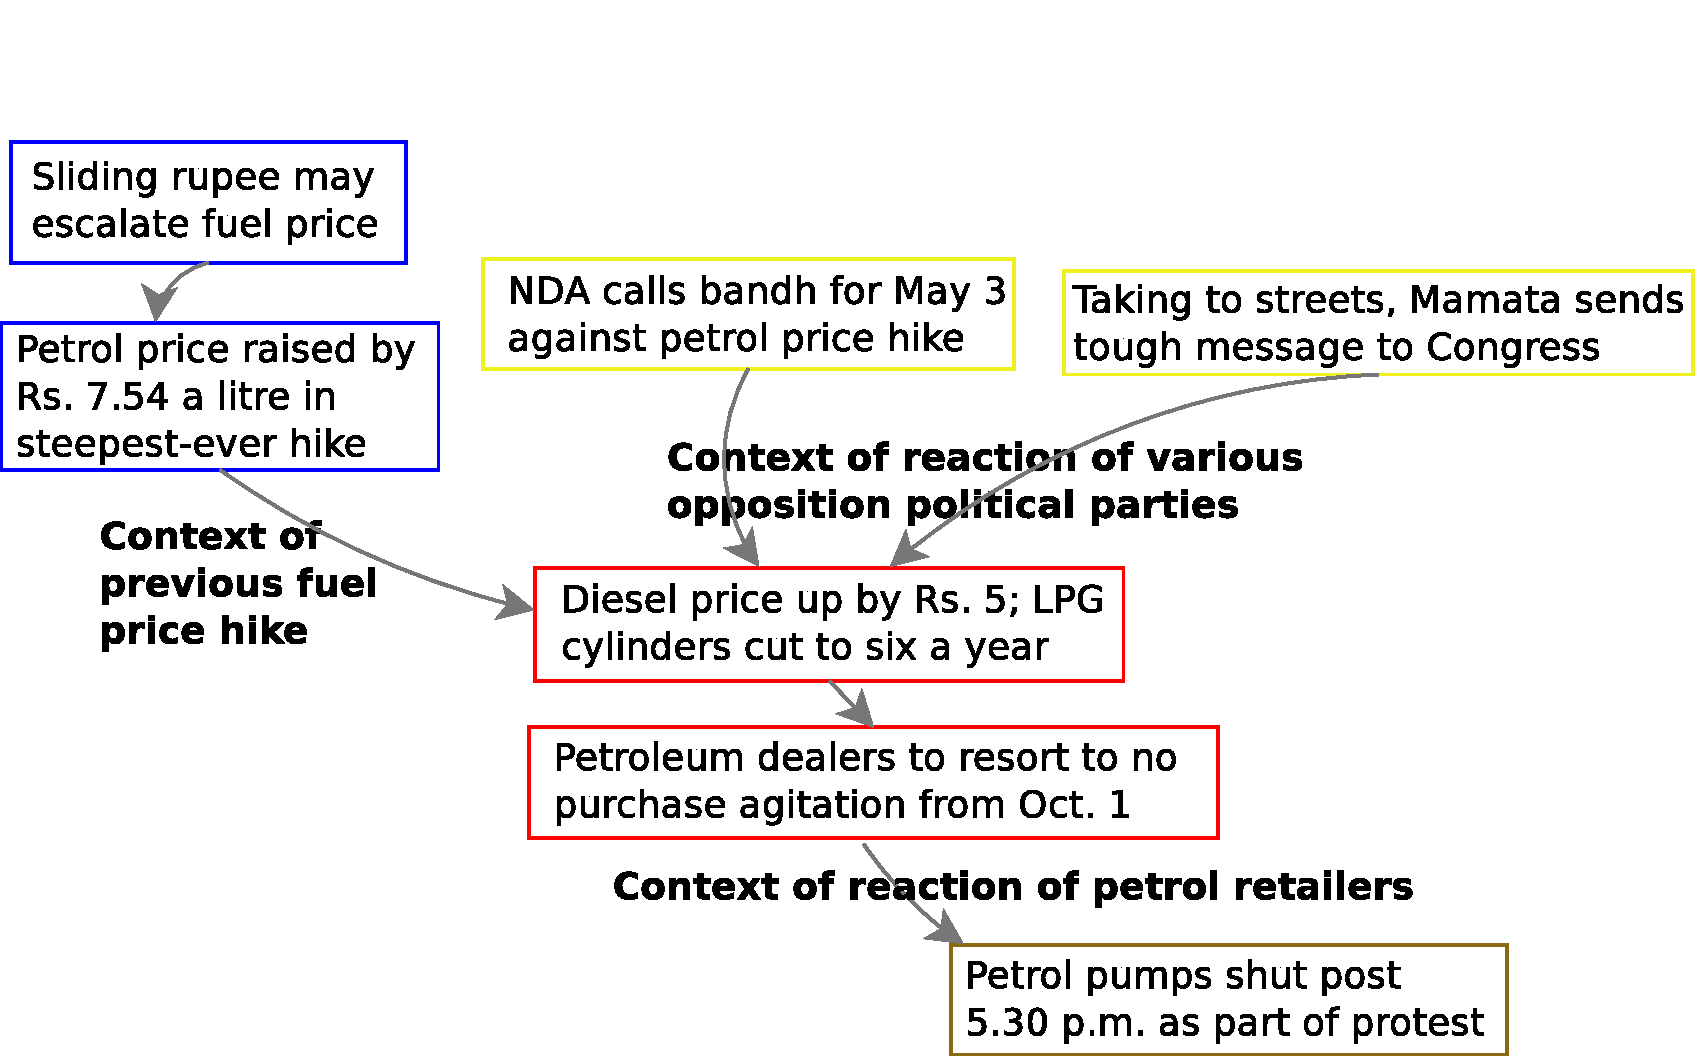
\includegraphics[scale=0.30]{figures/graph-petrol.pdf}
\label{fig:petrol}
\end{figure}

\subsubsection*{Overall article similarity}
\label{subsec:article_similarity}
The overall article similarity $r:\mathcal{A} \times \mathcal{A} \rightarrow [0,1]$ between 2 articles where $\mathcal{A}$ is the set of all articles is defined as:
\begin{equation}
r(a, b) = sim(a,b) * Jacc(\mathcal{E}(a), \mathcal{E}(b)) * e^{-\alpha|\tau_a - \tau_b|}
\end{equation}
Here, $sim$ is cosine similarity between articles represented as vectors in the TfIdf space, $Jacc$ is the jaccard similarity between
the entity sets of articles $a$ and $b$, and the final term is to factor in the time elapsed (in days) between their publishing dates ($\tau_a$ \& $\tau_b$).
The value of $\alpha$ was kept at 1. This score is pre-computed for each pair of articles. 

Next, we normalize each of these metrics to [0, 1] by dividing with the maximum score respective metric that is observed in the window defined by $[\tau - P, \tau + F]$. This
step is needed so we can compare these scores across different news stories. Our net score to bring out utility of presenting an article $b$ is the product of the 3 metrics.
\subsection{Context-extraction algorithm}
The setting is as follows: A user issues a certain filter query (like ``{\bf Corruption} AND {\bf Manmohan Singh}''). The result article set $S$ is computed by applying this filter on the news graph backend. Now, we want to identify articles
related to $S$ via a path in the graph, which would be helpful to the user to understand the story and the bigger picture.
Our algorithm can now be described as follows: We attempt to get ``most useful'' neighbourhood of $S$. The algorithm is a walk on the news graph starting from articles in $S$, 
going as far as till we get the desired number of stories to present to the user. This is similar to a user clicking ``Next'' at the bottom of a search results page to get more results. 

\begin{algorithmic}
  \State \textbf{\underline{GetNeighbourhood}}
  \State \algorithmicrequire{Input article set $S$, MaxStories $\theta$}
  \State \algorithmicensure{Neighbourhood $N$}
    \State $Q \leftarrow$ \{\} \Comment{Empty Priority Queue}
    \ForAll {node $n \in S$}
      \State Enqueue($Q$, ($n, 1$))
    \EndFor
    \While {Is\_Empty($Q$) == {\bf False} and $|N| \leq \theta$}
      \State $(v, w)$ = Dequeue($Q$)
      \State $N \leftarrow N \cup \{v\}$
      \ForAll {node $n \in Neighbours(v)$}
        \State $w_1 \leftarrow coh_{v}(n)$
        \State $w_2 \leftarrow cont_{S}(n)$
        \State $w_3 \leftarrow r(v,n)$
        \State $w_{eff} \leftarrow w_1 * w_2 * w_3 * w$
        \State Enqueue\_Or\_Update\_Node($Q$, ($n, w_{eff}$))
      \EndFor
    \EndWhile
    \State return $N$
\end{algorithmic}

Here, $Neighbours$ returns all of a node's neighbours in the graph. $Q$ is an object of priority queue ADT\footnote{Abstract Datatype} which was implemented as a heap. \emph{Enqueue} adds a node according to its weight to the heap. \emph{Enqueue\_Or\_Update\_Node} has the semantics that it updates the weight and position of node $n$ in $Q$ if found, else adds the node to $Q$.
\emph{Dequeue} returns the node with the highest weight in the heap. We call $GetNeighbourhood(S, \theta)$ where $S$ is the result set of a user's query and $\theta = 30$ for our experiments. The choice of $\theta$ is driven by the front-end interface, and we found 30 to work well.
The intuition behind this algorithm is that we want to identify those nodes from the neighbourhood of the result set $S$, which are both coherent and contextual to $S$, and do so in an efficient manner (variant of BFS on the graph).

\subsection{Some examples of context extracted}
In this section, we present sample news graphs generated on various stories and show how context is useful for each of them.

\begin{figure}
\caption{Robert Vadra corruption story and its contexts}
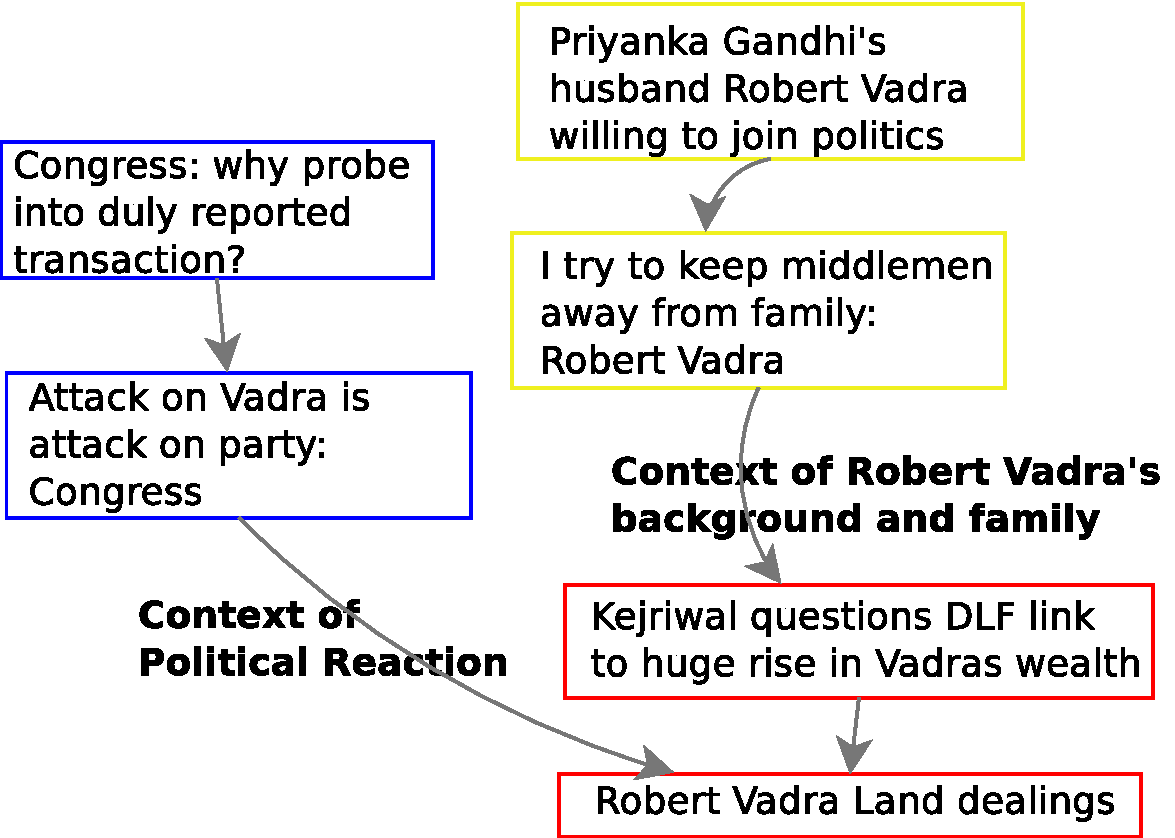
\includegraphics[scale=0.30]{figures/graph-vadra.pdf}
\label{fig:vadra-corruption}
\end{figure}

Consider Figure~\ref{fig:vadra-corruption} showing the graph of the story around Robert Vadra's alleged
corruption scandal reported in the news. As the story progresses in time, the articles
start to assume that the reader has enough knowledge of who Robert Vadra is, what is he known for,
how has this controversy spiralled to include the top political parties of India, etc. Hence, these articles
become increasingly inaccessible to a user with less prior context. However, 
using the graph, we can provide this context at any stage. Moreover, while following the story, 
the reader can look for how have the political parties reacted to this story as another context.
\begin{figure*}
\caption{A graph snippet showing multiple stories}
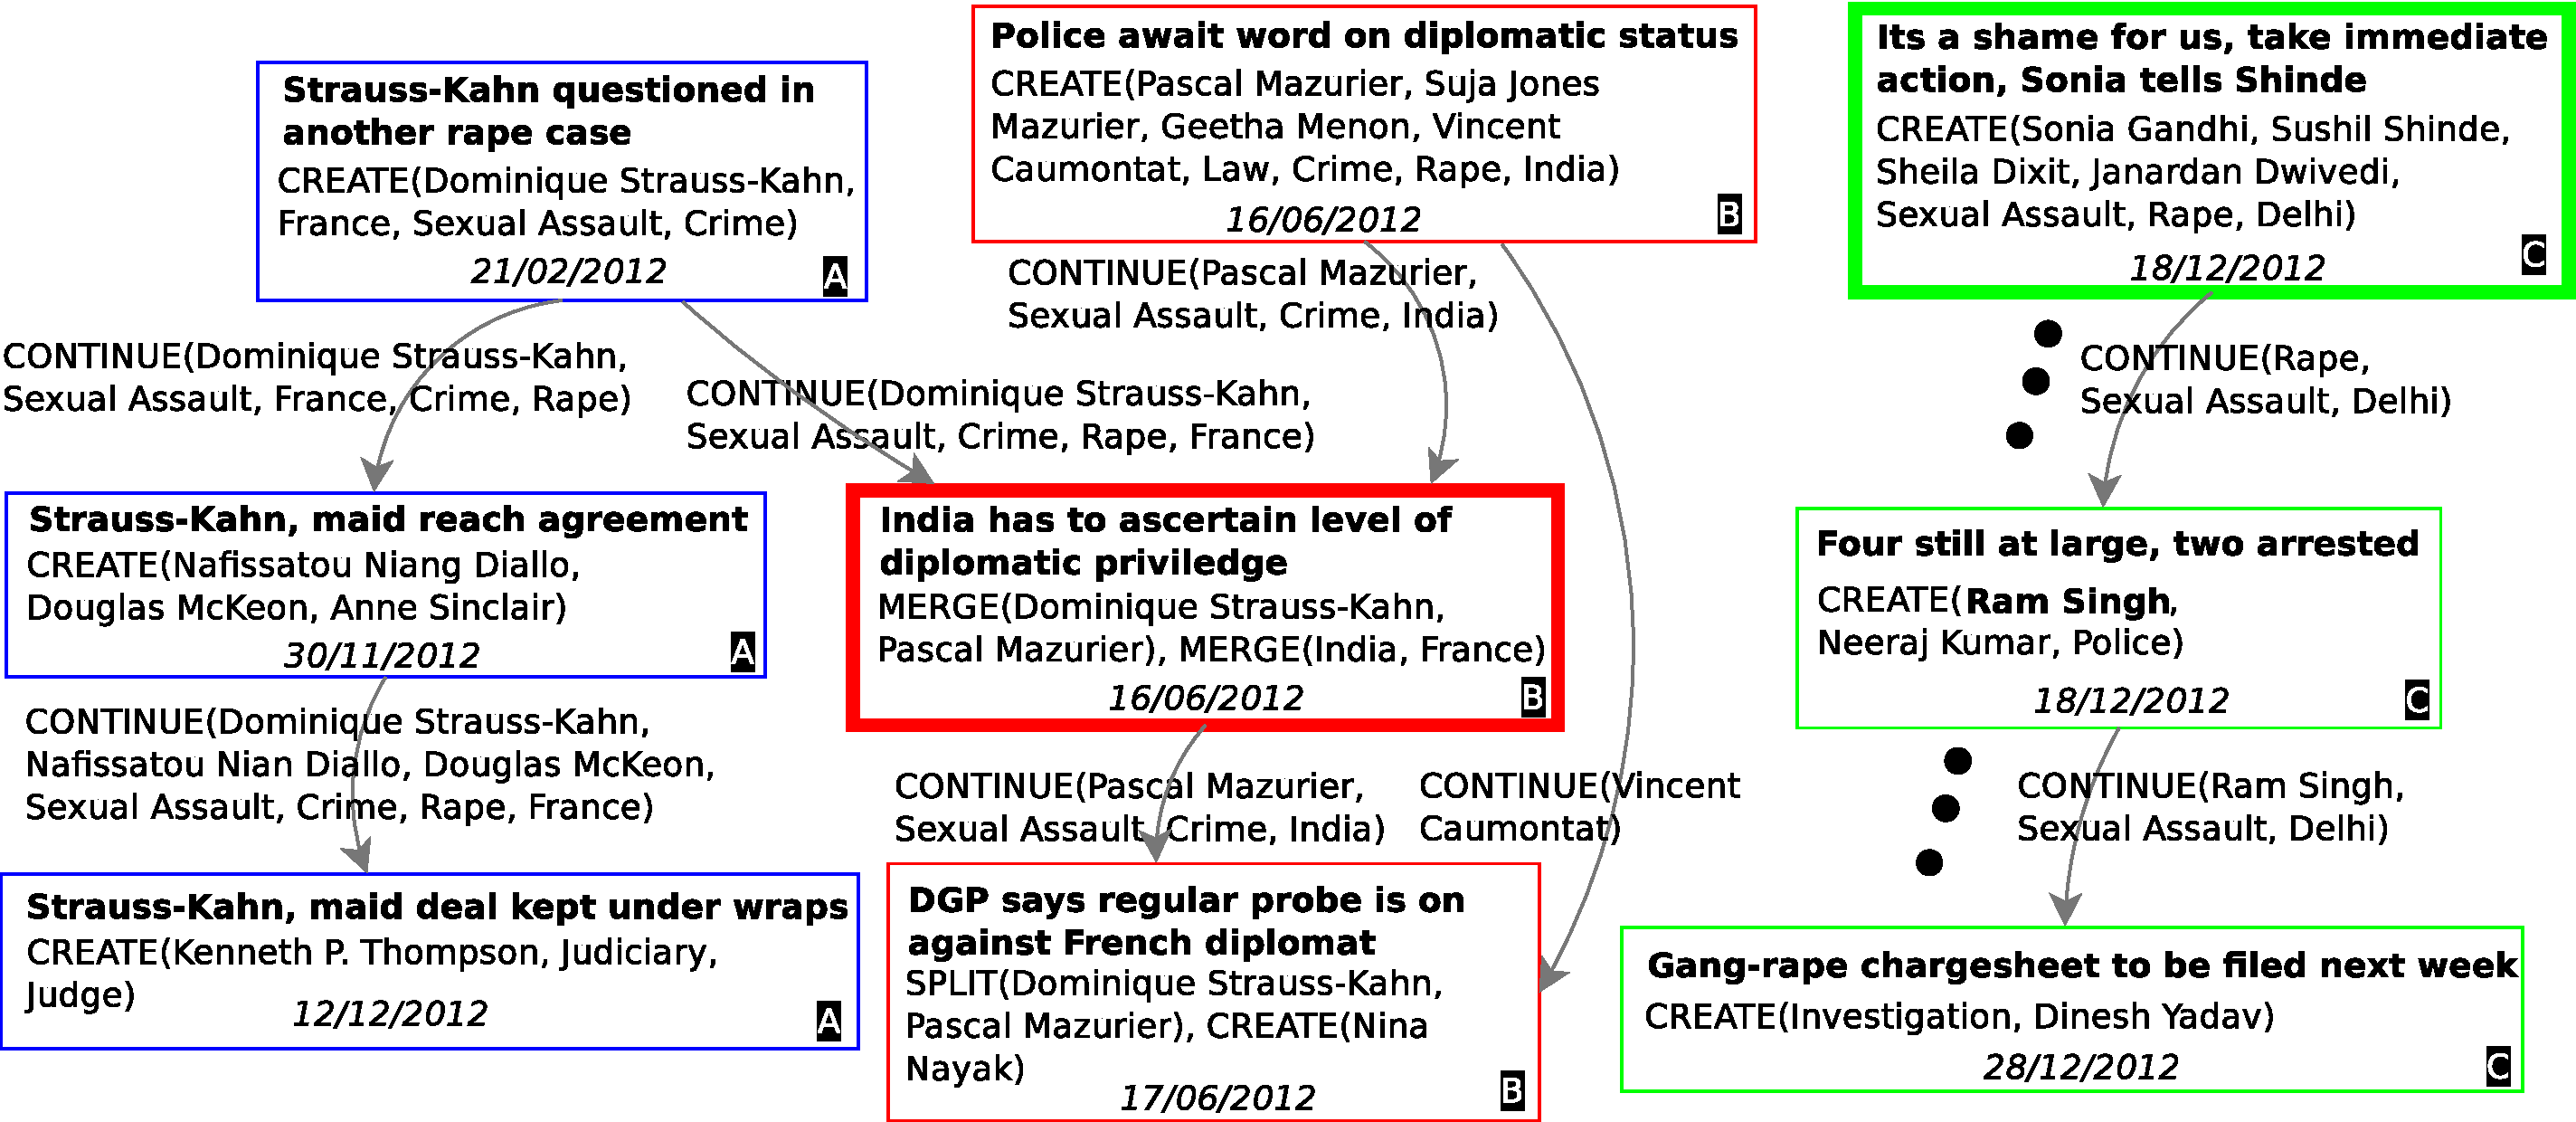
\includegraphics[scale=0.34]{figures/graph-2.pdf}
\label{fig:context-graph-example}
\end{figure*}

 

Consider Figure~\ref{fig:context-graph-example} where 3 distinct stories are presented. The nodes marked $A$(in blue) cover a case involving Dominique Strauss-Kahn (DSK), 
those marked $B$(in red) cover of a case surrounding Pascal Mazurier(PM), and those marked $C$(in green) talk of the internationally reported Gang-rape case
that happened in Delhi(DGR).\footnote{In no way do we want to use this unfortunate incident or others discussed in the paper in any way except 
to exemplify the technicalities of our work.} Two key things can be noted here. Even with a fair overlap of topics (Sexual Assault, Rape), the DSK and DGR subgraphs are not directly linked to each other.
On the other hand, the PM and DSK stories have a direct link in between them. This points to the fact, that the graph generation algorithm is successfully able
to determine how close or far stories (subgraphs) are to each other.

A key strength of our approach is that we allow the user to iteratively query the underlying corpus on multiple parameters and never have to recreate
the graph. Having created the graph once, we just filter out only the relevant nodes clusters and visualize them on a timeline as events. 
